\documentclass[tikz]{standalone}
\usepackage{tikz}
\usetikzlibrary{positioning}

\newcommand{\costs}{ \text{cost} }
\newcommand{\lightred}{white!60!red}
\newcommand{\partfrac}[2]{\frac{\partial #2}{\partial #1}}

\begin{document}
	
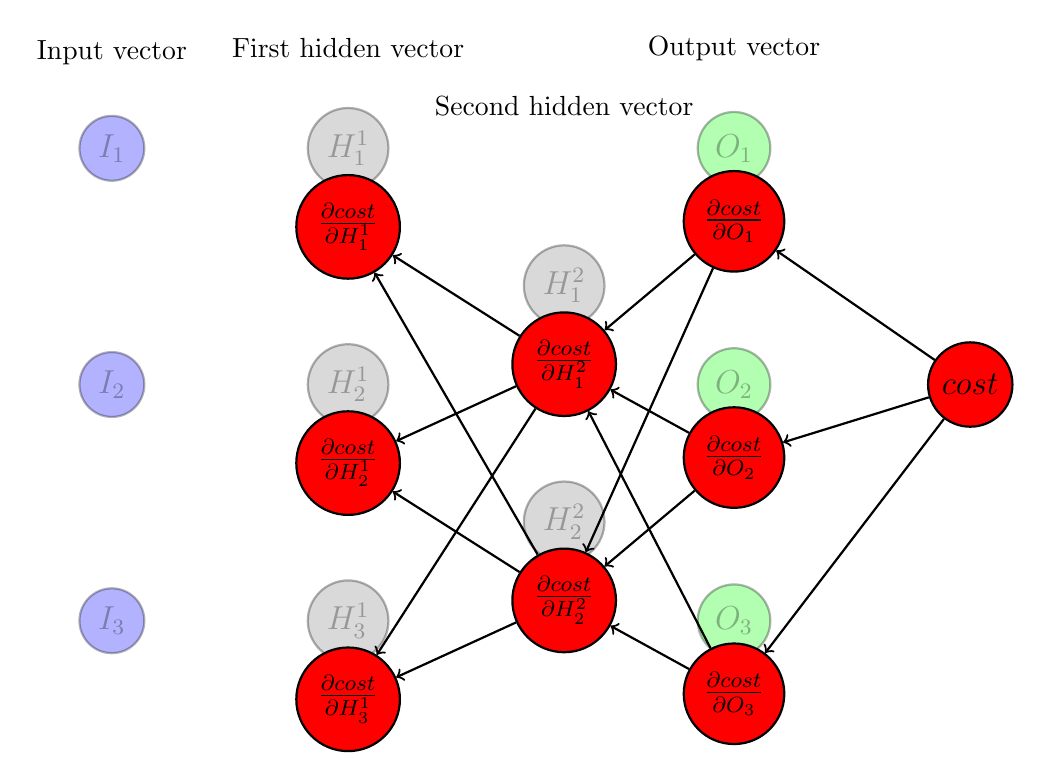
\begin{tikzpicture}[auto, node distance=3cm, every loop/.style={},
thick,main node/.style={circle,draw,font=\sffamily\large\bfseries}]

\node[main node] [fill=blue,opacity=0.3] [label={[shift={(0,0.5)}]Input vector}] (A) {$I_1$};
\node[main node] [fill=blue,opacity=0.3] (B) [below of=A] {$I_2$};
\node[main node] [fill=blue,opacity=0.3] (C) [below of=B] {$I_3$};
\node[main node] [fill=gray,opacity=0.3] [label={[shift={(0,0.5)}]First hidden vector}] (D) [right of=A] {$H^1_1$};
\node[main node] [fill=gray,opacity=0.3] (E) [right of=B] {$H^1_2$};
\node[main node] [fill=gray,opacity=0.3] (F) [right of=C] {$H^1_3$};
\node[main node] [fill=gray,opacity=0.3] [label={[shift={(0,1.5)}]Second hidden vector}] (G) [below right = 1cm and 2cm of D] {$H^2_1$};
\node[main node] [fill=gray,opacity=0.3] (H) [below right = 1cm and 2cm of E] {$H^2_2$};
\node[main node] [fill=green,opacity=0.3] (I) [label={[shift={(0,0.5)}]Output vector}] [right = 7cm of A] {$O_1$};
\node[main node] [fill=green,opacity=0.3] (J) [right = 7cm of B] {$O_2$};
\node[main node] [fill=green,opacity=0.3] (K) [right = 7cm of C] {$O_3$};
\node[main node] [fill=red] (L) [right of= J] {$\costs$};

\node[main node] [fill=red] (P)  [below = -0.2cm of I] {$\partfrac{O_1}{\costs}$};
\node[main node] [fill=red] (Q)  [below = -0.2cm of J] {$\partfrac{O_2}{\costs}$};
\node[main node] [fill=red] (R)  [below = -0.2cm of K] {$\partfrac{O_3}{\costs}$};
\node[main node] [fill=red] (S)  [below = -0.2cm of G] {$\partfrac{H^2_1}{\costs}$};
\node[main node] [fill=red] (T)  [below = -0.2cm of H] {$\partfrac{H^2_2}{\costs}$};
\node[main node] [fill=red] (U)  [below = -0.2cm of D] {$\partfrac{H^1_1}{\costs}$};
\node[main node] [fill=red] (V)  [below = -0.2cm of E] {$\partfrac{H^1_2}{\costs}$};
\node[main node] [fill=red] (W)  [below = -0.2cm of F] {$\partfrac{H^1_3}{\costs}$};


\foreach \x in {P,Q,R}
\path[every node/.style={font=\sffamily\normalsize}]
(L) [->] edge node [] {} (\x);
\foreach \x in {P,Q,R}
\foreach \y in {S,T}
\path[every node/.style={font=\sffamily\normalsize}]
(\x) [->] edge node [] {} (\y);

\foreach \x in {S,T}
\foreach \y in {U,V,W}
\path[every node/.style={font=\sffamily\normalsize}]
(\x) [->] edge node [] {} (\y);

\end{tikzpicture}

	
\end{document}